\section{First and Second Derivative Tests}
\subsection{First Derivative Test}
As we saw in previous sections, we can use the first derivative to find critical values, which allow us to find extrema.
\begin{theorem}[First Derivative Test]
	Let $f(x)$ be a continuous function.
	At a critical point $c$,
	\begin{enumerate}
		\item If $f^\prime$ changes sign from positive to negative ($f^\prime(x) > 0$ for $x < c$ and $f^\prime(x) < 0$ for $x > c$), then $f$ has a local maximum at $c$.
		\item If $f^\prime$ changes sign from negative to positive ($f^\prime(x) < 0$ for $x < c$ and $f^\prime(x) > 0$ for $x > c$), then $f$ has a local minimum at $c$.
		\item If $f^\prime$ does not change sign at $c$, then $f$ does not have a local extrema at $c$.
		\item At a left endpoint $a$, if ($f^\prime < 0$ / $f^\prime > 0$), then $f$ has a local (maximum / minimum) at $a$.
		\item At a right endpoint $b$, if ($f^\prime < 0$ / $f^\prime > 0$), then $f$ has a local (minimum / maximum) at $b$.
	\end{enumerate}
\end{theorem}

\begin{example}
	Find the local extrema of $f(x) = x^3 - 12x - 5$.
	Identify any absolute extrema.
\end{example}
\begin{answer}
	Taking the derivative,
	\begin{equation*}
		f^\prime(x) = 3x^2 - 12 = 3(x+2)(x-2).
	\end{equation*}
	
	So, the critical values are $x=-2$ and $x=2$.
	$f^\prime$ is negative between these values and positive outside of them, so $x=-2$ is a local maximum, while $x=2$ is a local minimum.
	\begin{equation*}
		f(-2) = 11 \text{ and } f(2) = -21.
	\end{equation*}
	
	As $x$ approaches $\infty$ (the right endpoint), $f$ also approaches $\infty$, so there is no absolute maximum.
	Similarly, as $x$ approaches $-\infty$ (the left endpoint), $f$ also approaches $-\infty$, so there is no absolute minimum.
\end{answer}

\subsection{Second Derivative Test}
The second derivative tells us how the derivative is changing.
Whether the derivative is increasing or decreasing describes the concavity.
\begin{definition}
	On some open interval $I$, the graph of a twice differentiable function $f(x)$ is
	\begin{enumerate}
		\item Concave up if $f^{\prime\prime} > 0$ on $I$.
		\item Concave down if $f^{\prime\prime} < 0$ on $I$.
	\end{enumerate}
\end{definition}


Concave up portions of a graph tend to look like valleys, while concave down portions tend to look like hills.
Unlike the first derivative, we can tell if a function is increasing or decreasing using concavity.
We can however say if the function is increasing or decreasing more or less rapidly.

\begin{figure}[H]
	\label{mvt}
	\centering
	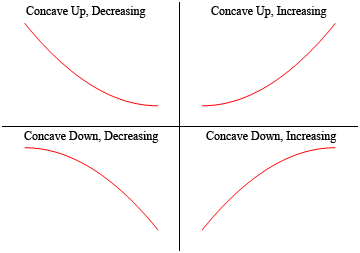
\includegraphics[width = 0.5\textwidth]{./applications_derivative/concavity.png}
	\caption{\hyperref{https://tutorial.math.lamar.edu/classes/calci/shapeofgraphptii.aspx}{}{}{Paul's Online Notes - The Shape of a Graph, Part II}}
\end{figure}


The points where a function changes concavity are called ``inflection points.''
At these points, the function is increasing or decreasing most rapidly, depending on the sign of the first derivative.


Rather than looking at the sign of $f^\prime$ around critical values, we can look at the concavity at the critical point.
\begin{theorem}[Second Derivative Test]
	Let $c$ be a critical value of $f$.
	\begin{enumerate}
		\item If $f^{\prime\prime}(c) < 0$, then $c$ is a local maximum.
		\item If $f^{\prime\prime}(c) > 0$, then $c$ is a local minimum.
		\item If $f^{\prime\prime}(c) = 0$, then the test is inclusive.
	\end{enumerate}
\end{theorem}

In other words, if we're at a critical point that's turning into a valley, then the critical point must be the top of a hill.
If we're at a critical point that's turning into a hill, then the critical point must be the bottom of a valley.
This test is particularly useful because you only need to know $f^{\prime\prime}$ at $c$ rather than an entire interval\footnote{It also extends to higher dimensions much better than the first derivative test.}.

\begin{example}
	Use the second derivative test to find the local extreme values of $f(x) = x^3 - 12x - 5$.
\end{example}
\begin{answer}
	Finding critical values,
	\begin{align*}
		f^\prime(x) &= 3x^2 - 12 = 3(x+2)(x-2). \\
		f^\prime(x) &= 0\text{ at } x=-2, x=2.
	\end{align*}
	
	Taking the second derivative,
	\begin{equation*}
		f^{\prime\prime}(x) = 6x.
	\end{equation*}
	
	Evaluating the second derivative at the critical values,
	\begin{equation*}
		f^{\prime\prime}(-2) = -12 \text{ and } f^{\prime\prime}(2) = 12.
	\end{equation*}
	
	So, $x=-2$ is a local maximum and $x=2$ is a local minimum.
\end{answer}